\section{Theorie}
\label{sec:Theorie}
\subsection{Zielsetzung}
In diesem Versuch sollen zunächst verschieden periodische elektrische
Schwingungen in ihre Fourier-Komponenten zerlegt werden. Anschließend sollen
ebendiese Funktionen wieder aus ihren theoretisch errechneten Anteilen
zusammengesetzt werden.

\subsection{Fouriere-Analyse}
Als periodische Funktionen werden jene Funktionen bezeichnet, welche nach
einer bestimmten Periodendauer T oder einer festen Distanz D erneut ihren
ursprünglichen Startwert annehmen, so dass
\begin{align}
  & f(t+T)=f(t) \\
  \text{und    }      & f(x+D)=f(x)
  \label{eqn:period}
\end{align}
gilt. Häufig auftretende Funktion sind hierbei Sinus- und Cosinusfunktion,
welche durch eine bestimmte Amplitude a bzw. b und eine Periodendauer T
charakterisiert sind.
Das Fouriersche Theorem besagt zudem, das ein Großteil der stetigen periodischen
Funktionen aus der Summation mehrer dieser Funktion zusammensetzen lässt gemäß
der Gleichung
\begin{equation}
   f(t)= \frac{1}{2}a_0 + \sum_{n=1}^\infty (a_n \cos n \frac{2 \pi}{T}t
   + b_n \sin n \frac{2 \pi}{T}t)
\end{equation}
wobei die Reihe gleichmäßig konvergent ist. Die entsprechenden Amplituden
berechnen sich durch
\begin{align}
  & a_n = \frac{2}{T} \int_0^T f(t) \cos n \frac{2 \pi}{T}t dt \\
  \text{und    }     & b_n = \frac{2}{T} \int_0^T f(t) \sin n \frac{2 \pi}
  {T}t dt
\end{align}
mit n $\in \symbb{N} $. Es treten dabei nur ganzzahlige Vielfache der
Grundfrequenz $v = \frac{1}{T} $ auf, welche auch als harmonische Oberwellen
bezeichnet werden. Trägt man diese gegen ihre jeweilige Amplitude auf, ergibt
sich daraus ein diskretes Linienspektrum, wie es in \ref{fig:spektrum} zu
sehen ist.
\begin{figure}[H]
  \centering
  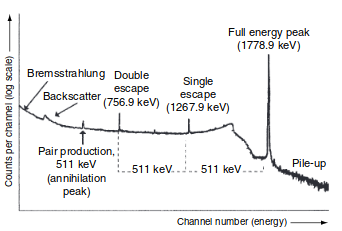
\includegraphics{Spektrum}
  \caption{Linienspektrum einer Fourier-Ananlyse \cite{skript}}
  \label{fig:Biegung}
\end{figure}
